\documentclass[a4paper,11pt]{article}
\usepackage{mystyle}
\usepackage[bottom]{footmisc}
\usepackage{mathrsfs}

\begin{document}

\section{Algorithme}
\label{algo}
\begin{enumerate}
\item
  Résoudre le problème aux valeurs propres pour trouver $(\lambda_i,\mbf{g}_i)_{i=1,\dots,M}$
\item
  Trouver les conditions aux bords $\alpha_i$ à la sortie. (sect \ref{cdtsortie})
\item
  Trouver le relévement des conditions aux bords $\mbf{a}$. (sect \ref{relev})
\item
  Ecrire Navier-Stokes pour $\mbf{v}=\mbf{a}+\mbf{u}$ où $\mbf{a}$ est connue et $\mbf{u}$ est l'inconnue.
  \begin{gather*}
    \frac{\partial \mbf{v}}{\partial t} + (\curl  \mbf{v})\times \mbf{v} + \grad q + \frac{1}{Re}\curll  \mbf{v}-\mbf{f} = 0\\
    \frac{\partial \mbf{u}}{\partial t} + (\curl \mbf{u})\times \mbf{u} + (\curl \mbf{u})\times \mbf{a} +(\curl \mbf{a})\times \mbf{u} + \grad q +\frac{1}{Re}\curll  \mbf{u} - \mbf{f_a} = 0\\
  \end{gather*}
  avec $\mbf{f_a}=\mbf{f}-\frac{\partial \mbf{a}}{\partial t} - (\curl \mbf{a})\times \mbf{a} - \curll\mbf{a}$
\item
  Injecter $\mbf{u}=\sum_{i=1}^\infty c_i(t)\mbf{g}_i(x,y,z)$ où $\mbf{g}_i$ sont connus et $c_i$ sont les inconnus.
  \begin{align*}
    \sum_{i=1}^\infty\frac{\partial c_i}{\partial t}\mbf{g}_i &+ \sum_{i=1}^\infty\sum_{j=1}^\infty c_i c_j((\curl\mbf{g}_i)\times \mbf{g}_j) + \sum_{i=1}^\infty c_i((\curl\mbf{g}_i)\times \mbf{a})\\
    & + \sum_{i=1}^\infty c_i((\curl\mbf{a})\times \mbf{g}_i) + \grad \pi_{\mbf{a}} +\frac{1}{Re}\sum_{i=1}^\infty c_i\curll\mbf{g}_i - \mbf{f_a} = 0
  \end{align*}
\item
  Formulation faible avec $\forall \varphi\in D^1 \Leftrightarrow \forall \mbf{g}_k\quad k=1,\dots,M$
  \begin{equation*}
    \frac{\partial c_k}{\partial t} + \frac{1}{Re}c_k\lambda_k^2 + \sum_{i=1}^M\sum_{j=1}^Mc_ic_jR_{ijk} + \sum_{i=1}^Mc_iR_{iak} + \sum_{i=1}^Mc_iR_{aik} = R_{fk}
  \end{equation*}
  avec :
  \begin{align*}
    R_{ijk} &= \int_\Omega((\curl\mathbf{g}_i)\times \mathbf{g}_j)\cdot\mathbf{g}_k & R_{iak} &= \int_\Omega((\curl\mathbf{g}_i)\times \mathbf{a})\cdot\mathbf{g}_k\\
    R_{aik} &= \int_\Omega((\curl\mathbf{a})\times \mathbf{g}_i)\cdot\mathbf{g}_k & R_{fk} &= \int_\Omega\mathbf{f_a}\cdot\mathbf{g}_k
  \end{align*}
\end{enumerate}

\section{Poiseuille}
On prend un écoulement de Poiseuille qui est solution de Navier-Stokes, avec le profil suivant : $\mbf{v} = (0,0, 2(1-\frac{x^2+y^2}{R^2}))$ dans un cylindre de rayon $R=0.5$ et de longueur $L=5$ pour un nombre de Reynolds de 1.\\
On a donc les conditions aux limites suivantes :
\begin{gather*}
  \alpha_0 = \mbf{v}\cdot\mbf{n} =
  \begin{cases}
    -\mbf{v}_z & \mbox{ sur } \Gamma_1\\
    +\mbf{v}_z & \mbox{ sur } \Gamma_2\\
    0 & \mbox{ sur } \Gamma_3
  \end{cases}\\
  \alpha_1 = \curl\mbf{v}\cdot\mbf{n} = 0 \mbox{ sur } \Gamma\\
  \alpha_2 = \curll\mbf{v}\cdot\mbf{n} =
  \begin{cases}
    -32 & \mbox{ sur } \Gamma_1\\
    +32 & \mbox{ sur } \Gamma_2\\
    0 & \mbox{ sur } \Gamma_3
  \end{cases}
\end{gather*}

On sait aussi que l'écoulement est stationnaire donc $\frac{\partial\mbf{v}}{\partial t}=0$.\\
De plus, le terme non linéaire de Navier-Stokes est nul, il reste donc
\begin{gather}
  \frac{1}{Re}\curll\mbf{v}=-\grad p\\
  \frac{1}{Re}\left( \int_\Omega(\curll\mbf{u})\cdot\mbf{g}_k  + \int_\Omega(\curll\mbf{a})\cdot\mbf{g}_k \right) = \int_\Omega p\div\mbf{g}_k - \int_\Gamma p\mbf{g}_k\cdot\mbf{n}
\end{gather}
On sait que $\mbf{g}_k\in D^1$ donc $\mbf{g}_k=\mbf{g}_k^0 + \grad\phi_k$,
en utilisant les formules de Green suivantes :
\[
\int_\Omega \curl\bm{\varphi}\cdot\bm{\psi} = \int_\Omega \bm{\varphi}\cdot\curl\bm{\psi} + \int_\Gamma (\mbf{n}\times\bm{\varphi})\cdot\bm{\psi}\quad\quad
\int_\Omega \bm{\varphi}\cdot\grad\psi = -\int_\Omega \psi\div\bm{\varphi} + \int_\Gamma \psi\bm{\varphi}\cdot\mbf{n}
\]
on a :
\[
\int_\Omega \curll\bm{\varphi}\cdot\mbf{g}_k = \int_\Omega \curl\bm{\varphi}\cdot\curl\mbf{g}_k^0 + \int_\Gamma \psi_k\curll\bm{\varphi}\cdot\mbf{n}
\]
d'ou
\begin{gather}
  \frac{1}{Re}\left( \int_\Omega(\curl\mbf{u})\cdot(\curl\mbf{g}_k)  + \int_\Omega(\curl\mbf{a})\cdot(\curl\mbf{g}_k) + \int_\Gamma \alpha_2\phi_k \right) = 0\\
  \frac{1}{Re}\sum_i c_i\lambda_i\lambda_k\int_\Omega \mbf{g}_i\cdot\mbf{g}_k = -\frac{1}{Re}\left( \int_\Omega (\curl\mbf{a})\cdot(\curl\mbf{g}_k) + \int_\Gamma \alpha_2\phi_k \right)\\
  c_k = -\frac{1}{\lambda_k^2}\left( \int_\Omega (\curl\mbf{a})\cdot(\curl\mbf{g}_k) + \int_\Gamma \alpha_2\phi_k \right)
\end{gather}

\subsection{Stokes}
Dans le cas où $\mbf{a} = \grad\psi^0$, on a que $\curl\mbf{a} = \curll\mbf{a} = 0$ et donc que $\mbf{u}$ doit être solution du problème de Stokes :
\begin{pb} Trouver $\mbf{u}\in D^1$ et $p\in H^1\setminus \R$ tel que :
  \begin{equation*}
    \left\{
    \begin{aligned}
      \curll\mbf{u} + \grad p &= 0 & \Omega\\
      \div \mbf{u} &= 0 & \Omega\\
      \curll\mbf{u}\cdot\mbf{n} &= \alpha_2 & \Gamma
    \end{aligned}
    \right.
  \end{equation*}
\end{pb}
Comme $\mbf{u}$ doit appartenir à $D^1$, on se sert de la matrice de changement de base utilisé pour le problème aux valeurs propres. Ceci nous permet d'imposer la condition $\curl\mbf{u}\cdot\mbf{n}=0$.\\
Pour imposer la divergence nulle, on utilise le terme de pression $p\in H^1\setminus \R$, que l'on choisit à moyenne nulle. Il faut donc aussi rajouter un multiplicateur de Lagrange.\\
On a donc la forme variationnelle suivante :
\begin{pb}Supposons $\mbf{b}\in [W^{-1/2,2}(\Gamma)]^3$. Trouver $(\mbf{u},p,\lambda)\in D^1\times H^1\setminus\R\times\R$ tel que :
  \begin{equation*}
    \underbrace{\int_\Omega \curl\mbf{u}\cdot\curl\bm{\phi}}_{A} + \underbrace{\int_\Omega \bm{\phi}\grad p}_{B^t} + \underbrace{\int_\Omega \mbf{u}\grad q}_{B} + \underbrace{\int_\Omega p\lambda}_\Lambda + \underbrace{\int_\Omega q\theta}_\Theta = \underbrace{- <\mbf{b}, \bm{\phi}>_\Gamma}_L
  \end{equation*}
  $\forall (\bm{\phi},q,\theta)\in D^1\times H^1\setminus\R\times\R$ avec $\bm{\phi}=\bm{\phi}_0+\grad\varphi$
\end{pb}
En utilisant les intégrations par parties, on sait que
\[<\mbf{b}, \bm{\phi}>_\Gamma=\int_\Gamma \varphi\underbrace{\curll\mbf{u}\cdot\mbf{n}}_{\alpha_2}\]

On obtient donc le problème sous forme matricielle suivant :
\begin{equation*}
  \begin{pmatrix}
    C^t & 0 & 0\\
    0 & Id & 0\\
    0 & 0 & Id
  \end{pmatrix}
  \begin{pmatrix}
    A & B^t & 0\\
    B & 0 & \Lambda\\
    0 & \Theta & 0
  \end{pmatrix}
  \begin{pmatrix}
    C & 0 & 0\\
    0 & Id & 0\\
    0 & 0 & Id
  \end{pmatrix}
  =
  \begin{pmatrix}
    C & 0 & 0\\
    0 & Id & 0\\
    0 & 0 & Id
  \end{pmatrix}
    \begin{pmatrix}
    L\\
    0\\
    0
  \end{pmatrix}
\end{equation*}
où C est la matrice de changement de base et
\begin{align*}
  A_{ij} &= \int_\Omega \curl\bm{\phi}_i\cdot\curl\bm{\phi}_j && i,j=1,\dots,M\\
  B_{ij} &= \int_\Omega \grad\psi_i\bm{\phi}_j && i=1,\dots,L\quad j=1,\dots,M\\
  \Lambda_i &= \int_\Omega \psi_i\lambda  && i=1,\dots,L\\
  \Theta_j &= \int_\Omega \psi_j\theta && j=1,\dots,L\\
  L_{i} &= <\mbf{b},\bm{\phi}_i>_\Gamma = \int_\Gamma \alpha_2\varphi_i && i=1,\dots,M
\end{align*}

Ce qui produit les résultats suivants :
\begin{figure}[H]
  \centering
  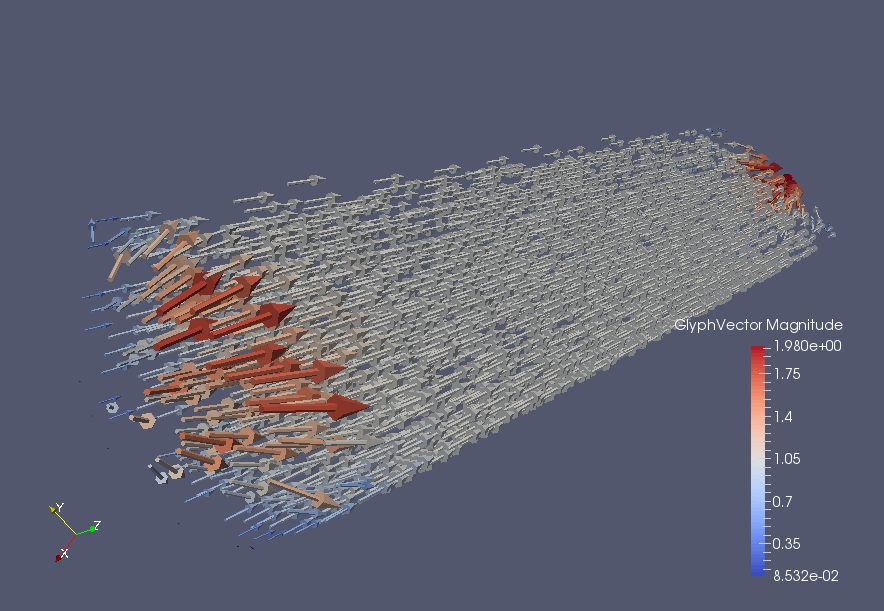
\includegraphics[scale=0.4]{aarrow}
  \caption{$\mbf{a}_h$ pour $h=0.05$}
\end{figure}
\begin{figure}[H]
  \centering
  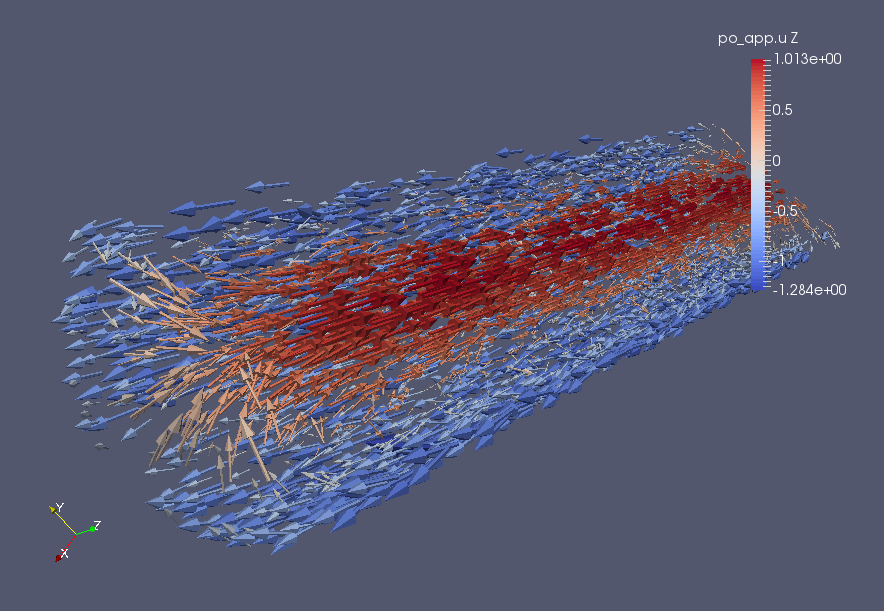
\includegraphics[scale=0.4]{uarrow}
  \caption{$\mbf{u}_h$ pour $h=0.05$}
\end{figure}
\begin{figure}[H]
  \centering
  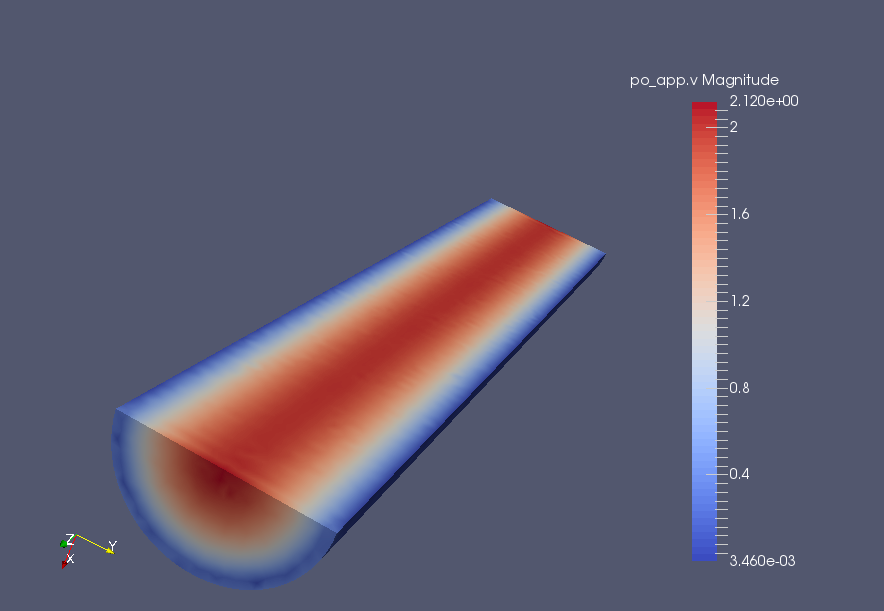
\includegraphics[scale=0.4]{vh}
  \caption{$\mbf{v}_h$ pour $h=0.05$}
\end{figure}
\begin{figure}[H]
  \centering
  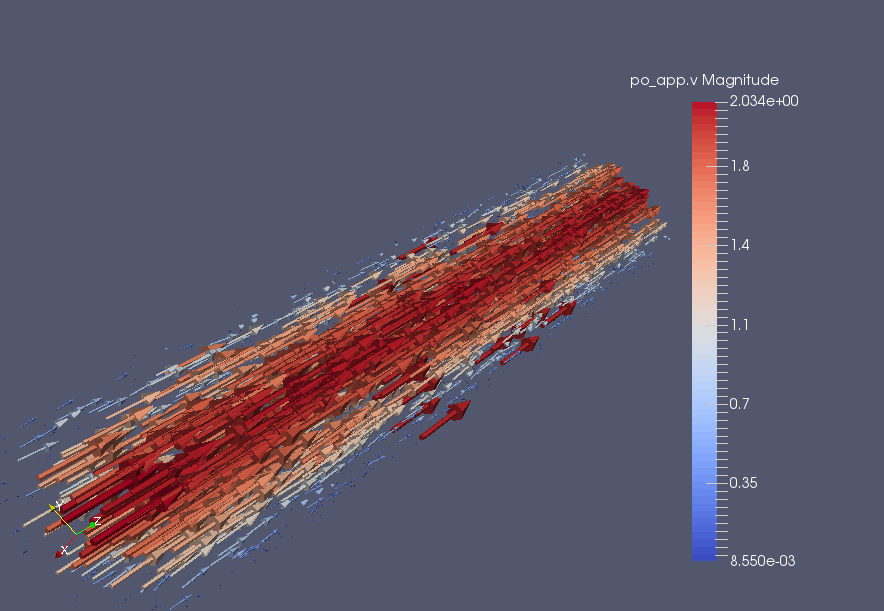
\includegraphics[scale=0.4]{vharrow}
  \caption{$\mbf{v}_h$ pour $h=0.05$}
\end{figure}

Avec les erreurs :
\begin{table}[H]
  \centering
  \begin{tabular}{c|c||c|c}
    h & \# Nh & $||\mbf{v}_h-\mbf{v}||_{L^2}$ & $||\curl\mbf{v}_h-\curl\mbf{v}||_{L^2}$ \\
    \hline
    0.1 & 20000 & 0.135 & 4.057\\
    0.05 & 200000 & 0.062 & 32.93
  \end{tabular}
\end{table}

Cela prouve donc que le rélévement de $\alpha_0$ et $\alpha_1$ fonctionne, sans avoir forcément à relever $\alpha_2$. Cette condition est imposée de manière faible lors de la résolution du problème.\\
On peut donc bien utiliser les fonctions propres avec le relévement proposé par P.Penel et J. Neustuppa pour résoudre le problème de Stokes.

\subsection{Fonctions propres}
\subsubsection{Stokes}
On résout donc le problème suivant :
\begin{pb}Trouver $\mbf{u}\in D^1$ tel que $\forall k=1,\dots,M$ :
  \[ \int_\Omega(\curl\mbf{u})\cdot(\curl\mbf{g}_k) = - \int_\Gamma \alpha_2\phi_k \]
  ce qui revient à trouver :
  \[ c_k = -\frac{1}{\lambda_k^2}\int_\Gamma \alpha_2\phi_k \]
\end{pb}

\begin{figure}[H]
  \centering
  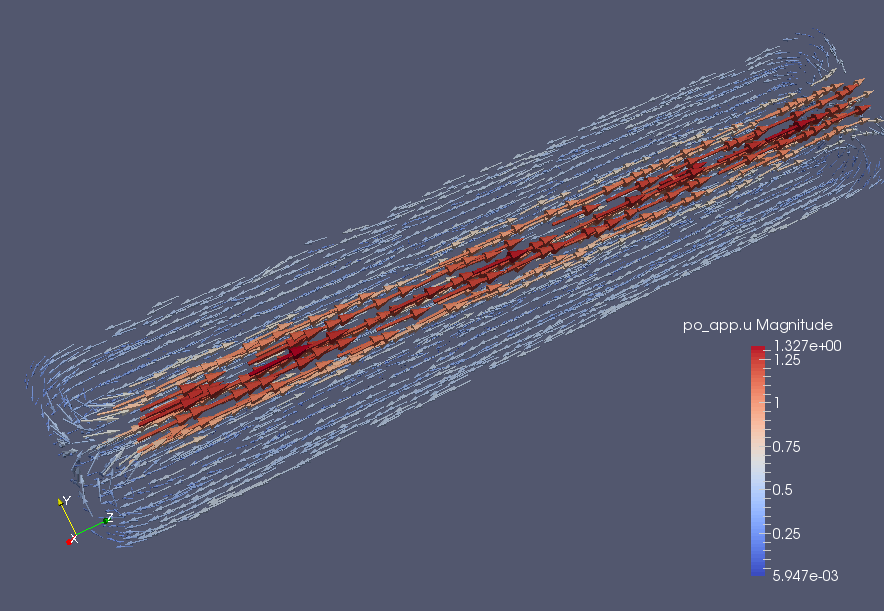
\includegraphics[scale=0.4]{u200}
  \caption{$\mbf{u}_h$ pour $h=0.075$ et 200 modes}
\end{figure}
\begin{figure}[H]
  \centering
  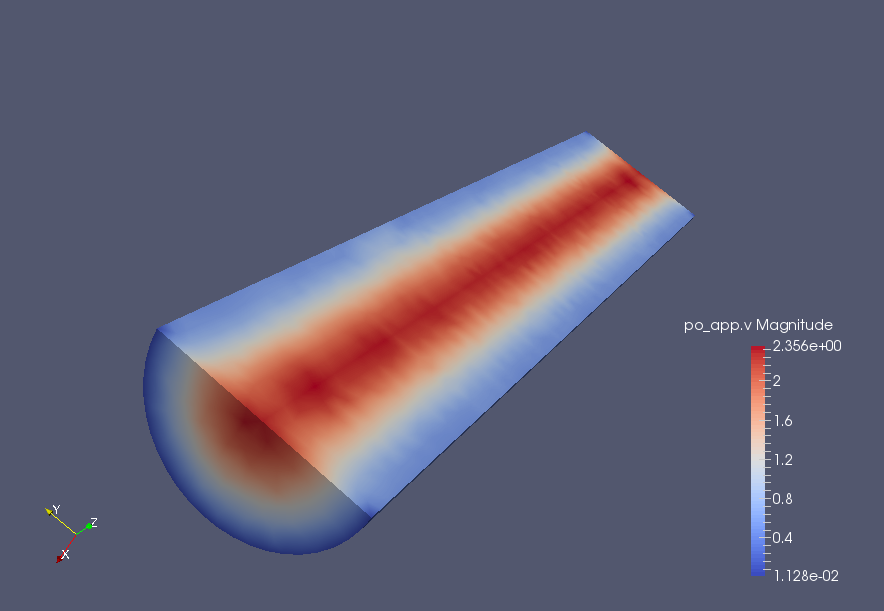
\includegraphics[scale=0.4]{v200}
  \caption{$\mbf{v}_h$ pour $h=0.075$ et 200 modes}
\end{figure}

L'erreur $||\mbf{v}_h - \mbf{v}||$ reste cependant vers 0.40, en augmentant le nombre de modes. Il faudrait donc utiliser une taille de maille plus petite.\\

La résolution de ce problème fonctionne donc mais présente certains inconvénients.
\begin{itemize}
\item
  La solution est plus sensible à la précision du relévement $\mbf{a}$.
\item
  Le problème aux valeurs propres demande une grande quantité de mémoire (plus de 400Go de RAM pour 200000 dofs)
\end{itemize}
Pour le premier, la résolution d'un système mixte, plutôt que deux problèmes successifs, pourrait améliorer la précision et la régularité de $\mbf{a} = \grad\phi^0$.\\
Pour le second, une idée est d'utiliser un préconditionneur pour le problème aux valeurs propres.\\
Au lieu de résoudre le problème $(Ax-\lambda Bx) = 0$, on résout $P^{-1}(Ax-\lambda Bx) = 0$ où le conditionnement de $P^{-1}A$ est meilleur que celui de $A$. Une difficulté pourait être de faire cohabiter le préconditionneur et la matrice de changement de base.\\
Mais appliquer d'abord le préconditionneur et ensuite le changement de base, devrait fonctionner, car une fois le précondionneur appliqué, les éléments se trouvent toujours dans $\N_h$ et donc, appliquer la matrice permet toujours de passer dans $\Z_h$.\\

L'idée est d'utiliser le préconditionneur définit dans \textit{Parallel numerical solution of the time-harmonic Maxwell equations in mixed form} par D. Li, G. Greif et D. Schötzau.\\

Ce qui devrait donner dans notre cas :
\[ C^t \mathscr{P}_M^{-1}ACx = \lambda C^t \mathscr{P}_M^{-1}BCx \]

\subsubsection{Navier-Stokes}
Pour Navier-Stokes on retrouve les mêmes résultats que précédemment, mais comme vu dans la section \ref{algo}, on doit calculer beaucoup de coefficients en plus.\\
Il y a $M^3 + M^2 + M^2 + M$ coefficients qui rentre en compte, mais en utilisant certaines propriétés de symétrie, on peut réduire ce nombre à $M^2(M-1)/2 + M^2 + M(M-1)/2 + M$.\\
Pour 100 modes propres, cela fait tout de même 510 050 coefficients à calculer.
Pour 86 modes et 325 467 coefficients, avec à peine plus de 10000 degrés de liberté sur 15 processeurs, cela prennait plus de 5h pour $R_{ijk}$, 450s pour $R_{aik}$ et $R_{iak}$ et quelques dizaines de seconde pour $R_{fk}$.\\
En utilisant des formes bilinéaires pour calculer ces coefficients, on arrive à 450s pour $R_{ijk}$, 6s pour $R_{aik}$, 12s pour, $R_{iak}$ et moins d'une seconde pour $R_{fk}$.\\
On arrive donc à une amélioration d'un facteur 40 pour le calcul de cette partie. Il y a encore peut-être une possibilité d'améliorer ce nombre pour $R_{ijk}$.

\section{Relévement}
\label{relev}
On suit ce qui est décrit dans l'article de J. Neustuppa et P. Penel\footnote{The Navier-Stokes equation with inhomogeneous boundary conditions based on vorticity, 2008} :

Pour relever $\alpha_1$, on utilise
\begin{equation}\label{a1}
  \left\{
  \begin{aligned}
    \bm{\psi}_1 - \grad p_1 &= 0 &\mbox{ sur }\Omega\\
    \div\bm{\psi}_1 &= 0 &\mbox{ sur }\Omega\\
    \bm{\psi}_1\cdot\mbf{n} &= \alpha_1 &\mbox{ sur }\Gamma
  \end{aligned}
  \right.
\end{equation}
et
\begin{equation}
  \left\{
  \begin{aligned}
    \curl\bm{\varphi}_0 &= \bm{\psi}_1 &\mbox{ sur }\Omega\\
    \bm{\varphi}_0 &= 0 &\mbox{ sur }\Gamma
  \end{aligned}
  \right.
\end{equation}

Puis pour $\alpha_0$ :
\begin{equation}\label{a0}
  \left\{
  \begin{aligned}
    \bm{\psi}_0 - \grad p_0 &= 0 &\mbox{ sur }\Omega\\
    \div\bm{\psi}_0 &= \div\bm{\varphi}_0 &\mbox{ sur }\Omega\\
    \bm{\psi}_0\cdot\mbf{n} &= \alpha_0 &\mbox{ sur }\Gamma
  \end{aligned}
  \right.
\end{equation}

Alors, $\mbf{a}=\bm{\varphi}_0+\bm{\psi}_0$.\\

Dans le cas où $\alpha_1=0$, on n'a plus qu'à résoudre \ref{a0} avec $\div\bm{\varphi}_0=0$, et alors $\mbf{a}=\bm{\psi}_0$.\\

Où les problèmes (\ref{a1}) et (\ref{a0}) sont des problèmes mixte de type Darcy que l'on peut résoudre à l'aide des éléments de Raviart-Thomas. Ce qui mène aux formulations faibles suivantes :\\
Trouver $(\bm{\psi}_i,p_i)\in \mathcal{U}\times\mathcal{Q}$ tel que :
\begin{equation}
  \int_\Omega\bm{\psi}_i\cdot\mbf{v} + \int_\Omega p_i(\div\mbf{v}) - \int_\Gamma p_i\mbf{v}\cdot\mbf{n} + \int_\Omega (\div\bm{\psi})q = \int_\Omega fq \quad \forall (\mbf{v},q)\in \mathcal{V}\times\mathcal{Q}
\end{equation}
où
\begin{gather*}
  \mathcal{U} = \{\mbf{u}\in H(\mathrm{div},\Omega) \;|\; \mbf{u}\cdot\mbf{n} = \alpha_i\}\\
  \mathcal{V} = \{\mbf{v}\in H(\mathrm{div},\Omega) \;|\; \mbf{v}\cdot\mbf{n} = 0\}\\
  \mathcal{Q} = \{p\in L_2(\Omega) \;|\; \int_\Omega p = 0 \}\\
  f=\begin{cases}
    0 &\mbox{pour } i=1\\
    \div\bm{\varphi}_0 &\mbox{pour } i=0
  \end{cases}
\end{gather*}

Pour augmenter la stabilité de la formulation, on utilise des termes supplémentaires définit dans l'article de M. R. Correa et A. F. D. Loula\footnote{Unconditionnaly stable mixed finite element methods for Darcy flow}. Parmi toutes les formulations proposées, j'ai choisi d'utiliser CGLS :
\begin{equation}
  \begin{aligned}
    \int_\Omega\bm{\psi}_i\cdot\mbf{v} &+ \int_\Omega p_i(\div\mbf{v}) + \int_\Omega (\div\bm{\psi}_i)q&\\
    &-\delta_1 \int_\Omega (\bm{\psi}_i-\grad p_i)\cdot(\mbf{v} +\grad q)&\\
    &-\delta_2 \int_\Omega \div\bm{\psi}_i\div\mbf{v}&\\
    &-\delta_3 \int_\Omega \curl\bm{\psi}_i\cdot\curl\mbf{v} &= \int_\Omega fq - \delta_2\int_\Omega f\div\mbf{v}
  \end{aligned}
\end{equation}

En choisissant $\delta_3=0$, on retrouve la formulation GCL(Hdiv) avec les estimations d'erreur suivantes :
\begin{gather}
  ||p-p_h||_1 \leq Ch^k(|\mbf{u}|_{k+1} + |p|_{k+1}),\\
  ||\mbf{u}-\mbf{u}_h|| \leq Ch^k(|\mbf{u}|_{k+1} + |p|_{k+1}),\\
  ||\div\mbf{u}-\div\mbf{u}_h|| \leq Ch^k(|\mbf{u}|_{k+1} + |p|_{k+1})
\end{gather}

\begin{tikzpicture}
  \begin{loglogaxis}[
      width=6.5cm,
      title=2D Convergence,
      xlabel=Mesh size ($h$),
      ylabel=$|| \mbf{u}-\mbf{u}_h ||_{L2}$,
      legend style = {legend pos = south east},
    ]
    \addplot table[x=hsize,y=l2err] {convergence2d_u.dat};
    \addplot[mark=none, style=dashed, forget plot] table[y = {create col/linear regression={y=l2err}}]{convergence2d_u.dat};
    \xdef \slope{\pgfplotstableregressiona};    
    \addlegendentry{P1 : $\pgfmathprintnumber{\slope}$}
  \end{loglogaxis}
\end{tikzpicture}
\hskip 10pt
\begin{tikzpicture}
  \begin{loglogaxis}[
      width=6.5cm,
      title=2D Convergence,
      xlabel=Mesh size ($h$),
      ylabel=$|| \div\mbf{u}-\div\mbf{u}_h ||_{L2}$,
      legend style = {legend pos = south east},
    ]
    \addplot table[x=hsize,y=l2err] {convergence2d_divu.dat};
    \addplot[mark=none, style=dashed, forget plot] table[y = {create col/linear regression={y=l2err}}]{convergence2d_divu.dat};
    \xdef \slope{\pgfplotstableregressiona};    
    \addlegendentry{P1 : $\pgfmathprintnumber{\slope}$}
  \end{loglogaxis}
\end{tikzpicture}

\begin{tikzpicture}
  \begin{loglogaxis}[
      width=6.5cm,
      title=2D Convergence,
      xlabel=Mesh size ($h$),
      ylabel=$|| p-p_h ||_{H1}$,
      legend style = {legend pos = south east},
    ]
    \addplot table[x=hsize,y=h1err] {convergence2d_p.dat};
    \addplot[mark=none, style=dashed, forget plot] table[y = {create col/linear regression={y=h1err}}]{convergence2d_p.dat};
    \xdef \slope{\pgfplotstableregressiona};    
    \addlegendentry{P1 : $\pgfmathprintnumber{\slope}$}
  \end{loglogaxis}
\end{tikzpicture}
\hskip 10pt
\begin{tikzpicture}
  \begin{loglogaxis}[
      width=6.5cm,
      title=3D Convergence,
      xlabel=Mesh size ($h$),
      ylabel=$|| p-p_h ||_{H1}$,
      legend style = {legend pos = south east},
    ]
    \addplot table[x=hsize,y=l2err] {convergence3d_p.dat};
    \addplot[mark=none, style=dashed, forget plot] table[y = {create col/linear regression={y=l2err}}]{convergence3d_p.dat};
    \xdef \slope{\pgfplotstableregressiona};    
    \addlegendentry{P1 : $\pgfmathprintnumber{\slope}$}
  \end{loglogaxis}
\end{tikzpicture}

\begin{tikzpicture}
  \begin{loglogaxis}[
      width=6.5cm,
      title=3D Convergence,
      xlabel=Mesh size ($h$),
      ylabel=$|| \mbf{u}-\mbf{u}_h ||_{L2}$,
      legend style = {legend pos = south east},
    ]
    \addplot table[x=hsize,y=l2err] {convergence3d_u.dat};
    \addplot[mark=none, style=dashed, forget plot] table[y = {create col/linear regression={y=l2err}}]{convergence3d_u.dat};
    \xdef \slope{\pgfplotstableregressiona};    
    \addlegendentry{P1 : $\pgfmathprintnumber{\slope}$}
  \end{loglogaxis}
\end{tikzpicture}
\hskip 10pt
\begin{tikzpicture}
  \begin{loglogaxis}[
      width=6.5cm,
      title=3D Convergence,
      xlabel=Mesh size ($h$),
      ylabel=$|| \div\mbf{u}-\div\mbf{u}_h ||_{L2}$,
      legend style = {legend pos = south east},
    ]
    \addplot table[x=hsize,y=l2err] {convergence3d_divu.dat};
    \addplot[mark=none, style=dashed, forget plot] table[y = {create col/linear regression={y=l2err}}]{convergence3d_divu.dat};
    \xdef \slope{\pgfplotstableregressiona};    
    \addlegendentry{P1 : $\pgfmathprintnumber{\slope}$}
  \end{loglogaxis}
\end{tikzpicture}

On voit donc que pour les cas tests, on a les ordres de convergence attendus.\\
Pour le relévement de $\alpha_0$, on ne connait ni le potentiel, ni le champ exact. Les quantités d'intérêts sont donc la divergence et la composante normale du champ.

\begin{tikzpicture}
  \begin{loglogaxis}[
      width=6.5cm,
      title=Composante normale,
      xlabel=Mesh size ($h$),
      ylabel=$|| \alpha_0-\mbf{a}_h\cdot\mbf{n} ||_{L2(\Gamma_1)}$,
      legend style = {legend pos = south east},
    ]
    \addplot table[x=hsize,y=an] {convergence_a.dat};
    \addplot[mark=none, style=dashed, forget plot] table[y = {create col/linear regression={y=an}}]{convergence_a.dat};
    \xdef \slope{\pgfplotstableregressiona};    
    \addlegendentry{P1 : $\pgfmathprintnumber{\slope}$}
  \end{loglogaxis}
\end{tikzpicture}
\hskip 10pt
\begin{tikzpicture}
  \begin{loglogaxis}[
      width=6.5cm,
      title=Divergence,
      xlabel=Mesh size ($h$),
      ylabel=$|| \div\mbf{a}_h ||_{L2}$,
      legend style = {legend pos = south east},
    ]
    \addplot table[x=hsize,y=div] {convergence_a.dat};
    \addplot[mark=none, style=dashed, forget plot] table[y = {create col/linear regression={y=div}}]{convergence_a.dat};
    \xdef \slope{\pgfplotstableregressiona};    
    \addlegendentry{P1 : $\pgfmathprintnumber{\slope}$}
  \end{loglogaxis}
\end{tikzpicture}

Un inconvénient à cette méthode est la visualisation des champs vectoriels utilisant les éléments de Raviart-Thomas. 

\begin{figure}[H]
  \centering
  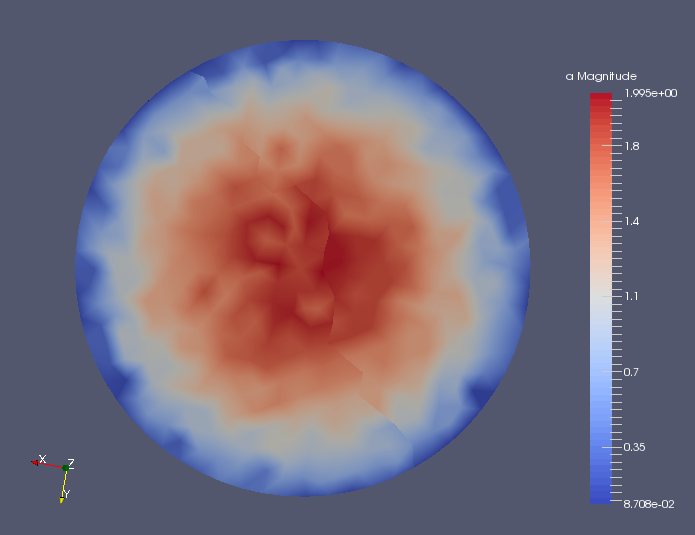
\includegraphics[scale=0.5]{aRT}
  \caption{Z-component with $h=0.05$ and 319343 dofs}
\end{figure}


\subsection{Conditions aux bords}
\label{cdtsortie}
Sur $\Gamma_3$ :
\[ \alpha_i=0\quad i=0,1,2\quad \Longrightarrow\quad \mbf{a}=\begin{pmatrix}0\\0\\0\end{pmatrix}\quad \Longrightarrow\quad \mbf{v}=\mbf{u} \]
\begin{equation}\label{base}
  \mbox{Dans la base }
  \begin{pmatrix}
    \bm{\tau}_1\\\bm{\tau}_2\\\mbf{n}
  \end{pmatrix}
  \quad\quad \mbf{v}=
  \begin{pmatrix}
    \frac{\partial\varphi}{\partial y}\\-\frac{\partial\varphi}{\partial x}\\0
  \end{pmatrix}
\end{equation}
$\mbf{v}$ est solution de Navier-Stokes :
\[ \frac{\partial\mbf{v}}{\partial t} + (\mbf{v}\cdot\nabla)\mbf{v} + \grad p - \frac{1}{Re}\laplace\mbf{v} - \mbf{f} = 0 \]
Et donc des deux équations suivantes :
\begin{gather}
  \frac{\partial\mbf{v}_x}{\partial t} + \mbf{v}_x\frac{\partial\mbf{v}_x}{\partial x} + \mbf{v}_y\frac{\partial\mbf{v}_x}{\partial y} + \frac{\partial p}{\partial x} + \frac{1}{Re}\left(\frac{\partial^2\mbf{v}_x}{\partial x^2} + \frac{\partial^2\mbf{v}_x}{\partial y^2}\right) - \mbf{f}_x = 0 \label{NS1}\\
  \frac{\partial\mbf{v}_y}{\partial t} + \mbf{v}_x\frac{\partial\mbf{v}_y}{\partial x} + \mbf{v}_y\frac{\partial\mbf{v}_y}{\partial y} + \frac{\partial p}{\partial y} + \frac{1}{Re}\left(\frac{\partial^2\mbf{v}_y}{\partial x^2} + \frac{\partial^2\mbf{v}_y}{\partial y^2}\right) - \mbf{f}_y = 0 \label{NS2}
\end{gather}

En dérivant (\ref{NS1}) par rapport à $y$ et (\ref{NS2}) par rapport à $x$, puis en soustrayant et en utilisant (\ref{base}), on obtient :
\begin{equation}
  \frac{\partial}{\partial t}\left(\grad^2\varphi\right) + \frac{\partial\varphi}{\partial y}\frac{\partial}{\partial x}\left(\grad^2\varphi\right) - \frac{\partial\varphi}{\partial x}\frac{\partial}{\partial y}\left(\grad^2\varphi\right) = \frac{1}{Re}\nabla^4\varphi
\end{equation}

Avec des conditions aux limites à définir, on peut donc connaître $\mbf{v}=\mbf{u}$ sur $\Gamma_3$ et donc sur $\partial\Gamma_2 = \Gamma_3\cap\Gamma_2$ le bord de $\Gamma_2$.\\

De plus, en supposant les vecteurs $\bm{\tau}_1$ et $\bm{\tau}_2$ orientés comme il faut, on a :\\
Dans la base correspondant à $\Gamma_3$ :
\[
\mbf{v}\restr{\Gamma_3\cap\Gamma_2} =
\begin{pmatrix}
  \mbf{v}_1\\\mbf{v}_2\\0
\end{pmatrix}=
\begin{pmatrix}
  \frac{\partial\varphi}{\partial y}\\-\frac{\partial\varphi}{\partial x}\\0
\end{pmatrix}
\]
Dans la base correspondant à $\Gamma_2$ :
\[
\quad\mbf{v}\restr{\Gamma_2\cap\Gamma_3} =
\begin{pmatrix}
  0\\\mbf{v}_1\\\mbf{v}_2(=\alpha_0)
\end{pmatrix} =
\begin{pmatrix}
  0\\\frac{\partial\varphi}{\partial y}\\-\frac{\partial\varphi}{\partial x}
\end{pmatrix}
\]

Une idée de Benjamin pour retrouver les $\alpha_i$ à la sortie est de trouver une fonction permettant de passer de $\alpha_0\restr{\Gamma_{1,3}}$ à $\alpha_0\restr{\Gamma_{2,3}}$ et de s'en servir pour passer de $\alpha_0\restr{\Gamma_1}$ à $\alpha_0\restr{\Gamma_2}$.\\
Cette fonction reste encore à déterminer.

\end{document}
